\documentclass[11pt,a4paper]{article}
\usepackage[margin=2.4cm]{geometry}
\usepackage{booktabs,graphicx,xcolor,amsmath,amssymb,longtable}
\usepackage[hidelinks]{hyperref}
\usepackage{sectsty}
\definecolor{acc}{HTML}{2C7FB8}
\sectionfont{\color{acc}}\subsectionfont{\color{acc}}
\setlength{\parskip}{4pt}\setlength{\parindent}{0pt}
\newcommand{\gene}[1]{\textit{#1}}
\title{\vspace{-1.5cm}\textbf{The Kingman \textit{et al.} 2021 stickleback dataset}\\[2pt]
\large Acquisition, packaging, and overlap with the 3sp LD-aware outlier regions}
\author{LDscnR-paper $\cdot$ \texttt{kingman2021/}}
\date{August 2026}

\begin{document}\maketitle

\section{Purpose}

This module acquires and packages the data of Roberts Kingman \textit{et al.} 2021,
\textit{Predicting future from past: the genomic basis of recurrent and rapid stickleback
evolution}, Sci Adv 7:eabg5285, as the \textbf{clear-peak} counterpart to the
\textbf{saturated} 3sp dataset already analysed in \texttt{module\_sticklebacks\_LDscnR/}.

3sp is the case where the whole genome carries real outlier regions and there is no
neutral floor. What the C-score machinery still needs is a dataset with a genuinely quiet
background against which the detectability gate and the negative-control-floor
$\tau_C$ calibration can be exercised. Kingman 2021 supplies exactly that: recurrent
marine$\rightarrow$freshwater adaptive loci standing sharply above a quiet background,
with a published, independently derived peak set to score against.

\section{Acquisition}

\subsection{The processed VCF exists, so no variant calling was needed}

The paper's Data Availability statement offers only raw SRA reads
(PRJNA247503: 1758 runs, 206 individuals, 0.7\,TB) and a track hub at
\texttt{sbwdev.stanford.edu}, which is dead --- no ICMP reply and TCP timeouts on both 80
and 443, from this network and through an off-network proxy.

However, the hub description page at
\url{https://web.stanford.edu/group/kingsley/hubDescription.html} notes that the entire
assembly hub is mirrored on \textbf{FigShare project 162634}. That mirror contains
\texttt{227\_genomes.final.filtered.vcf.gz} (15.3\,GB $+$ \texttt{.tbi}): a GATK-called,
VQSR-filtered joint VCF of all 227 genomes, already in gasAcu1-4 coordinates. The whole
alignment-and-calling path was therefore superseded and never run.

\subsection{Sources that could not be used}

\textbf{Dryad} (\texttt{10.5061/dryad.pvmcvdnjm}, \texttt{10.5061/dryad.547d7wm6t}) now
returns \texttt{\{"error":"Unauthorized, must have current bearer token"\}} from its API,
and its web download route sits behind an Anubis anti-bot challenge, which was not
circumvented. The reference genome was obtained from FigShare instead. Still unobtained
are the 363-SNP genotyping array and the published liftOver chains; neither is needed ---
the array is a validation panel rather than discovery data, and the chains were
reconstructed (\S\ref{sec:lift}). \textbf{science.org} blocks scripted access, so Table S2
was retrieved through a browser session.

\section{The dataset}

\subsection{Cohorts are one genome per population}

This is the design fact that governs everything downstream. The 227 genomes are
\emph{not} population samples; for the EcoPeak analyses they are one individual per
population, and Table S2 encodes the cohort membership, with the flag value being the
ecotype ($1$ = marine, $0$ = freshwater) and blank meaning "not in this cohort".

\begin{table}[h]\centering\small
\begin{tabular}{llrrl}\toprule
Cohort & Geography & $n$ & M / F & Published peak set \\ \midrule
\texttt{c155\_global} & global & 84 & 28 / 56 & Global specific: 39 peaks, 3.74\,Mb (0.8\% of genome) \\
\texttt{c150\_pacNW}  & N.E.\ Pacific & 68 & 11 / 57 & Pacific specific: 209 peaks, 27.4\,Mb (5.9\%) \\
\texttt{c151\_nEur}   & N.\ Europe & 27 & 9 / 18 & \textcolor{red}{none published} \\ \bottomrule
\end{tabular}
\end{table}

The \texttt{c155} membership reproduces the hub's stated "56 freshwater and 28 marine"
exactly, and all 227 Table S2 \texttt{Sequence ID}s match the 227 VCF sample names by set
equality. Every published peak-set region count and span was checked against the paper and
matches (39/3.7\,Mb, 209/27.4\,Mb, 212/91.9\,Mb).

\subsection{Coverage and the consequences of it}

Mean sequencing coverage is 5.5$\times$. At \texttt{MAF}$\,\geq0.05$ and
\texttt{F\_MISSING}$\,\leq0.20$, roughly 12\% of genotype calls are missing, and tightening
the filter is not an escape: \texttt{F\_MISSING}$\,\leq0.05$ retains only 3.8\% of SNPs.
The packaged \texttt{GTs} matrices are therefore \textbf{mean-imputed and numeric} rather
than integer $0/1/2$, because \texttt{gcta\_grm()} and \texttt{emmax\_setup()} have no NA
handling. Per-SNP \texttt{f\_missing} is carried in \texttt{map} so any downstream step can
filter on it. The residual caveat is real and should be remembered when interpreting
LD-based results: hard calls at 5.5$\times$ attenuate $r^2$ and hence \texttt{ld\_w}
relative to a high-coverage dataset. The VCF retains \texttt{PL}, so genotype-posterior
dosages remain available if attenuation proves limiting.

\subsection{Packaged bundles}

\begin{table}[h]\centering\small
\begin{tabular}{lrrl}\toprule
Bundle & Individuals & SNPs & Ecotype \\ \midrule
\texttt{kingman2021\_c155\_global.rds} & 84 & 3{,}509{,}797 & 28 M / 56 F \\
\texttt{kingman2021\_c150\_pacNW.rds}  & 68 & 4{,}073{,}192 & 11 M / 57 F \\ \bottomrule
\end{tabular}
\end{table}

Each is \texttt{list(GTs, map, eco, meta, cohort, source)} with \texttt{map} =
\texttt{marker, Chr, chr\_num, Pos, rec\_rate, cM, af, f\_missing}. \texttt{rec\_rate} is
the Rabbit Slough LDhelmet map in cM/Mb and \texttt{cM} its running integral; the map covers
96.4\% of SNPs, the remainder falling in gaps and carrying \texttt{NA}. A matched
\texttt{\_truth.rds} carries the peak table and per-SNP peak membership, row-aligned with
\texttt{map}.

\subsection{The packaged data reproduces the published peaks}

Naive $|\Delta\text{AF}|$ between ecotypes, inside the specific EcoPeaks versus the rest of
the genome:

\begin{table}[h]\centering\small
\begin{tabular}{lrrrr}\toprule
Cohort & median in-peak & background & above background 99.9th pct & Enrichment \\ \midrule
\texttt{c155\_global} & 0.179 & 0.058 & 29.8\% vs 0.10\% & \textbf{298$\times$} \\
\texttt{c150\_pacNW}  & 0.196 & 0.088 & 1.61\% vs 0.10\% & 16$\times$ \\ \bottomrule
\end{tabular}
\end{table}

And the background really is quiet, which is the property the dataset was acquired for: on
chrI:1--3\,Mb, which contains no EcoPeak, \textbf{0 of 24{,}551 SNPs} reach $p<10^{-6}$ and
8 reach $p<10^{-4}$ in an uncorrected ecotype regression, with $\lambda \approx 1.17$.

\textbf{Use \texttt{c155\_global} as the primary clear-peak dataset}: balanced 28/56 design
and a truth set covering only 0.8\% of the genome. \texttt{c150\_pacNW} is the secondary,
offering more truth regions but only 11 marine individuals.

\section{The coordinate bridge}\label{sec:lift}

3sp is in \textbf{gasAcu1} (\texttt{Chr1..Chr21}, arabic); everything Kingman is in
\textbf{gasAcu1-4} (\texttt{chrI..chrXXI}, roman). Since the published chains were
unobtainable, a chain was reconstructed from the hub's \texttt{bigChain} $+$
\texttt{bigChain.link} tracks (1{,}095 chains, 19{,}851 blocks) and reversed with UCSC
\texttt{chainSwap}.

It validates cleanly. Every peak set lifts at $\approx$100\% with preserved span
(c155 specific $3.743 \rightarrow 3.743$\,Mb; c150 specific $27.44 \rightarrow 27.18$\,Mb;
c150 sensitive $91.90 \rightarrow 90.69$\,Mb with 2 unmapped), chromosome assignment is
preserved throughout, and the \gene{Eda} EcoPeak at chrIV:12{,}795{,}310--12{,}892{,}195
lands at chrIV:12{,}782{,}916--12{,}879{,}801 --- a 12\,kb shift, as expected for two
near-identical assemblies on that chromosome.

\section{Overlap with the 3sp outlier regions}

The comparison target is the 40 LFMM outlier regions from
\texttt{module\_sticklebacks\_LDscnR} at $\tau_C = 0.05$, $l_{\min} = 10$,
$\rho_{ld} = 0.60$, spanning 21.13\,Mb (5.6\% of the SNP-covered genome).

\begin{table}[h]\centering\small
\begin{tabular}{lrrrrr}\toprule
Kingman set & Peaks & Genome & Regions hitting $\geq$1 peak & Fold & $p$ \\ \midrule
Global specific   & 36  & 0.9\%  & 4/40 (10\%)  & 1.38$\times$ & 0.33 \\
Global sensitive  & 83  & 5.8\%  & 13/40 (32\%) & 1.85$\times$ & \textbf{0.0065} \\
Pacific specific  & 193 & 6.6\%  & 15/40 (38\%) & 1.47$\times$ & \textbf{0.029} \\
Pacific sensitive & 189 & 21.7\% & 18/40 (45\%) & 1.13$\times$ & 0.29 \\ \bottomrule
\end{tabular}
\end{table}

Null is a within-chromosome shuffle of the regions, $B=2000$. By base pairs the picture is
similar: 2.3\% of LFMM span sits inside global-specific peaks against 0.9\% expected
(2.48$\times$, $p=0.08$). Reciprocally only 4 of 36 global-specific and 29 of 193
pacific-specific peaks are hit.

\textbf{This is a weak correspondence}, and the metrics disagree on significance. The
explanation turns out to be geography rather than method failure (\S\ref{sec:geo}).

\begin{figure}[h]\centering
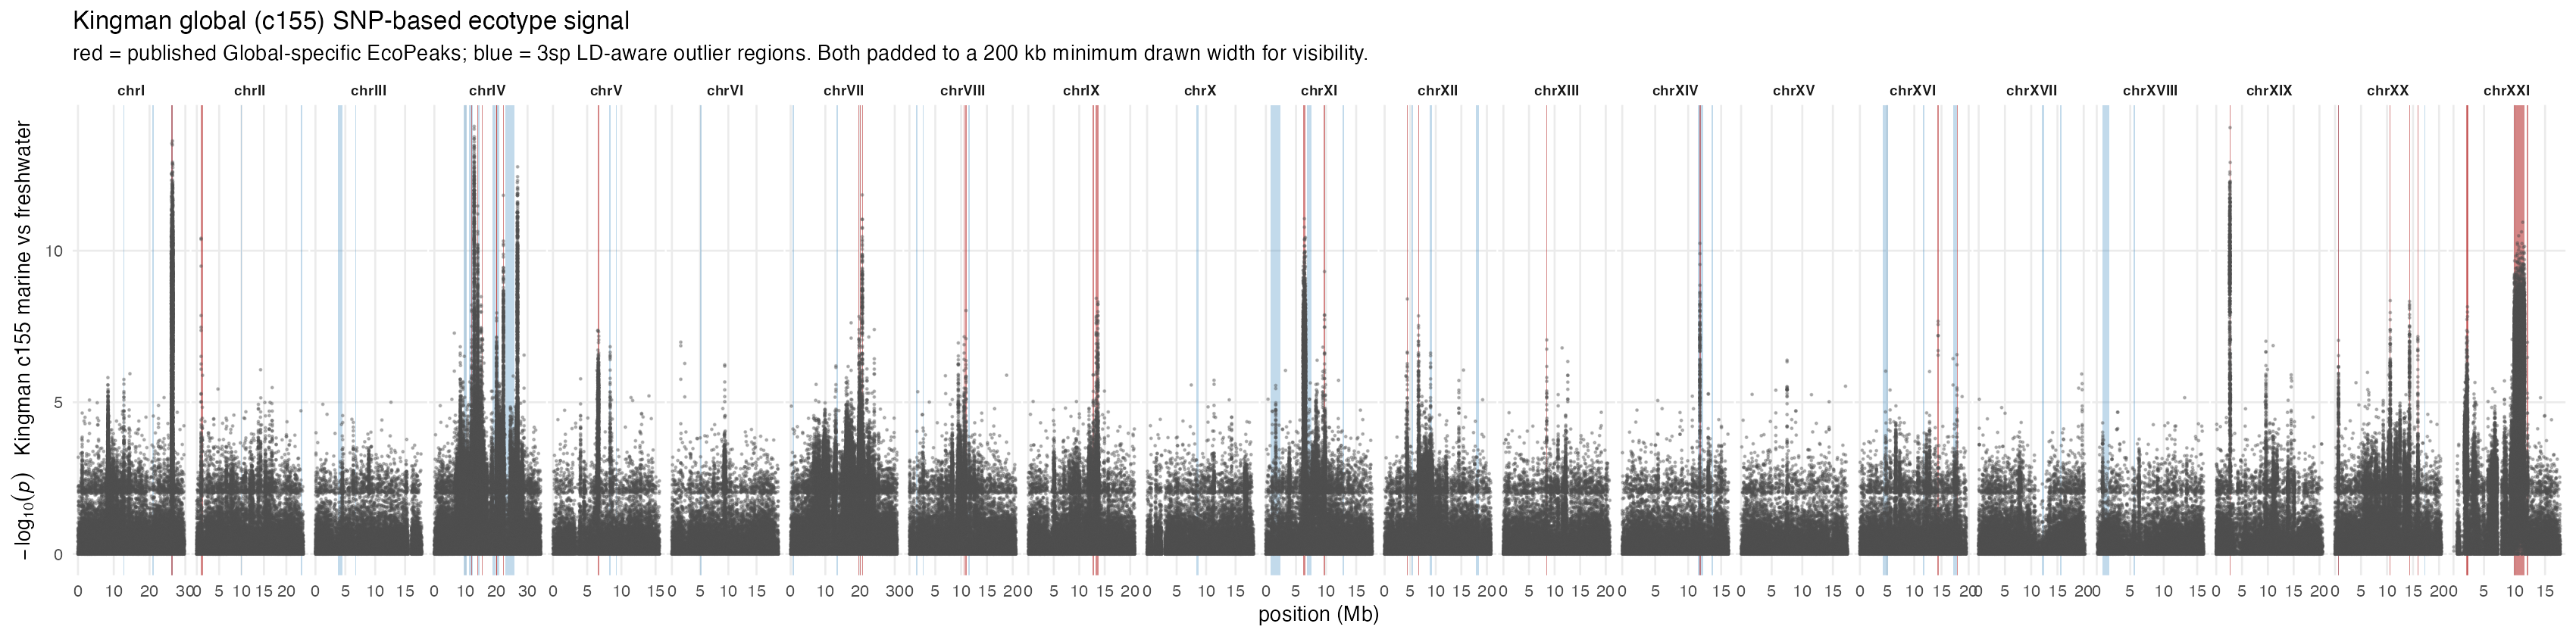
\includegraphics[width=\textwidth]{../figures/fig1_c155_manhattan_with_regions.png}
\caption{Kingman c155 SNP-based ecotype signal genome-wide. Red bands are the published
Global-specific EcoPeaks; blue bands are the 3sp LD-aware outlier regions lifted into
gasAcu1-4. Both are padded to a 200\,kb minimum \emph{drawn} width, since the median
global-specific peak is 21\,kb and would otherwise be sub-pixel; the data are unpadded.
Their limited coincidence is the observation this report explains.}
\end{figure}

\section{Re-deriving the Northern-European (c151) peak set}

\subsection{Method and validation}

Kingman used two methods, intersected at 1\% FDR for "specific" calls and unioned at 5\%
for "sensitive". Only the \textbf{SNP-based} test is specified precisely enough to
reproduce: holding the genotype-class totals $(n_0,n_1,n_2)$ and the marine group size $m$
fixed, the marine ALT-allele count is scored against a multivariate-hypergeometric null,
\[
P(a_0,a_1,a_2)=\frac{\binom{n_0}{a_0}\binom{n_1}{a_1}\binom{n_2}{a_2}}{\binom{N}{m}},
\qquad k=a_1+2a_2 ,
\]
two-sided on $|k - \mathbb{E}[k]|$. The null depends only on $(n_0,n_1,n_2,m)$, so it is
computed once per distinct key and cached; that is what makes it tractable genome-wide.
The companion window/CSS method is \textbf{not} implemented, since the published
description does not give the CSS formula.

The implementation was validated against both published cohorts:

\begin{table}[h]\centering\small
\begin{tabular}{llrl}\toprule
Cohort & Threshold & My peaks & Published \emph{specific} recovered \\ \midrule
\texttt{c155\_global} & BH $q\leq0.01$   & 286 / 15.5\,Mb & \textbf{36/39 (92\%)} \\
\texttt{c155\_global} & BH $q\leq10^{-4}$ & 46 / 3.83\,Mb  & 34/39 (87\%); 46/46 of mine hit a published peak \\
\texttt{c150\_pacNW}  & BH $q\leq10^{-4}$ & 274 / 35.2\,Mb & \textbf{195/209 (93\%)} \\ \bottomrule
\end{tabular}
\end{table}

At $q\leq10^{-4}$ the c155 output (46 peaks, 3.83\,Mb) is near-identical in size to the
published specific set (39 peaks, 3.74\,Mb). Because only one of the two methods is
implemented, these sets are a sensitive superset rather than a reproduction of "specific".

\begin{figure}[h]\centering
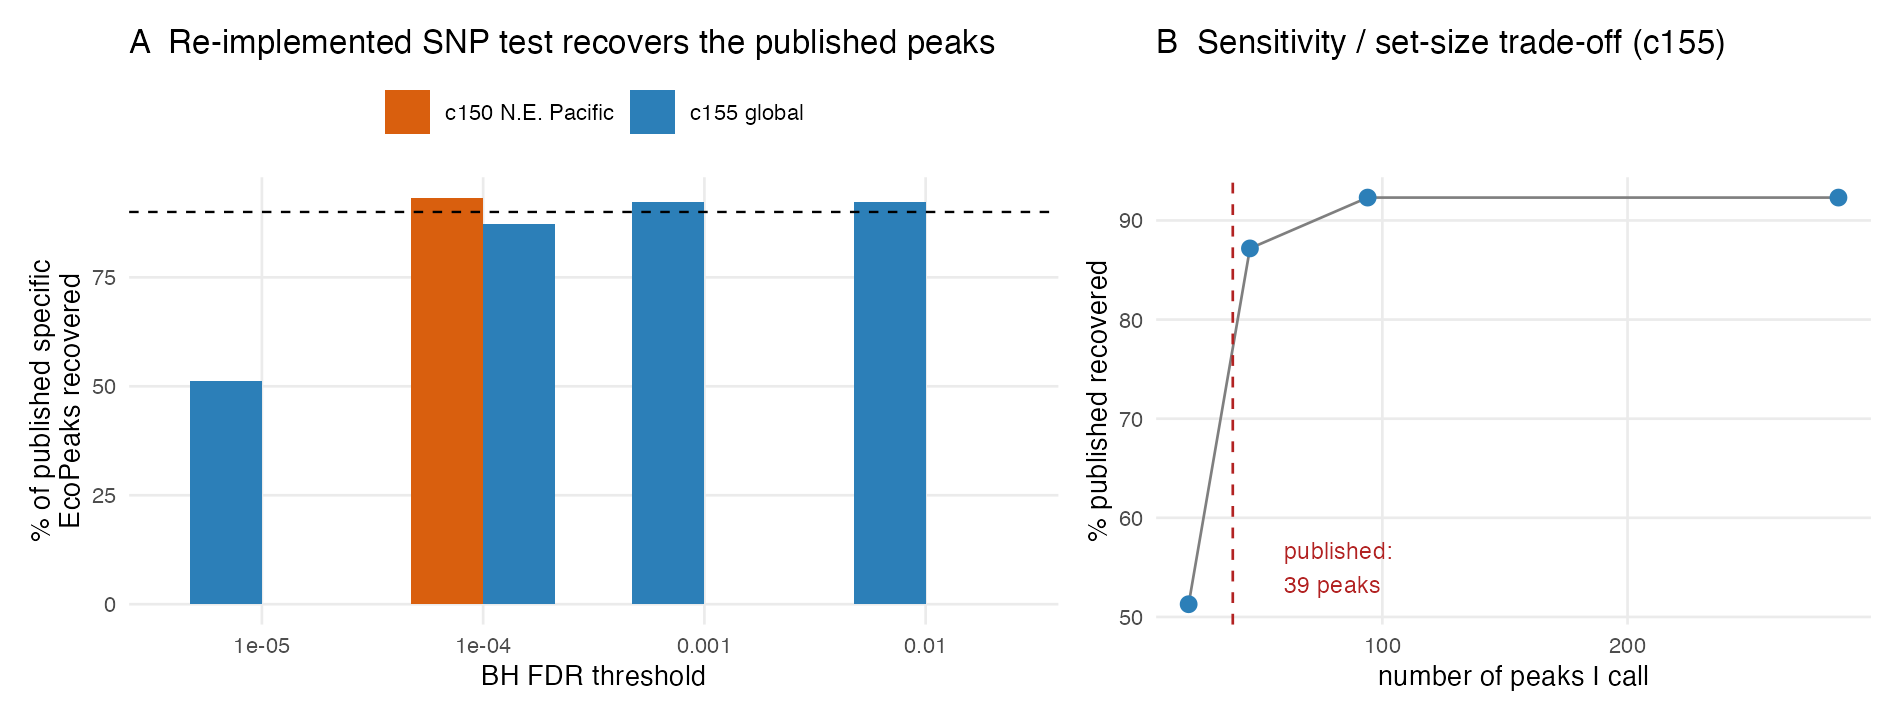
\includegraphics[width=\textwidth]{../figures/fig2_validation.png}
\caption{Validation of the re-implemented SNP-based test against the published peak sets.}
\end{figure}

\subsection{c151 cannot reach genome-wide significance, and this is structural}

c151 has 9 marine and 18 freshwater individuals, and after missingness the median marine
count actually called is \textbf{7} (range 2--9). The exact test therefore bottoms out at
$p = 3.2\times10^{-7}$, attained by exactly one SNP, whereas BH at $q\leq0.01$ over
1.70\,M tests would require $\geq54$ SNPs at that floor. \textbf{No SNP is significant at
any FDR}, and no threshold choice repairs it.

This is very likely why the hub publishes EcoPeak BEDs for c150 and c155 only, even though
Table S2 also defines c151, c153 and c154 cohorts. It is a property of the cohort, not of
the re-implementation --- which recovers 92--93\% of the published peaks where power exists.

What remains usable is the \emph{ranked} signal. A rank-based, explicitly
\textbf{not FDR-controlled} set was emitted from the top 0.1\% of $p$: 1{,}770 SNPs
$\rightarrow$ \textbf{41 suggestive peaks, 1.31\,Mb}.

\section{The geographic gradient}\label{sec:geo}

Ranks sidestep the significance floor entirely. Testing whether the 3sp outlier regions
(4.6--4.8\% of tested SNPs) are enriched for low Kingman $p$, with a within-chromosome
shuffle null:

\begin{table}[h]\centering\small
\begin{tabular}{llrrrr}\toprule
Kingman cohort & vs 3sp geography & top 1\% & $p$ & top 0.1\% & $p$ \\ \midrule
\texttt{c151} N. Europe    & \textbf{matches}   & \textbf{4.64$\times$} & \textbf{0.0040} & 1.07$\times$ & 0.28 \\
\texttt{c155} Global       & partial            & 3.19$\times$ & 0.024 & 6.30$\times$ & 0.0080 \\
\texttt{c150} N.E. Pacific & different basin    & 1.47$\times$ & 0.22  & 0.71$\times$ & 0.39 \\ \bottomrule
\end{tabular}
\end{table}

Independently, 11 of the 41 c151 suggestive peaks fall inside a 3sp outlier region against
2.80 expected: \textbf{3.93$\times$, $p = 0.0002$} (\texttt{R/11\_c151\_peak\_overlap.R}).

3sp is an entirely northern-European Atlantic panel --- lineage \texttt{NO}, sampled from
the Baltic, North Sea, Norwegian Sea and White Sea, 90 freshwater and 27 marine. The
published EcoPeaks it was first compared against are largely Pacific. Matching the ocean
basin roughly triples the agreement. \textbf{The weak headline overlap is geography, not a
failure of the LD-aware method.}

\begin{figure}[h]\centering
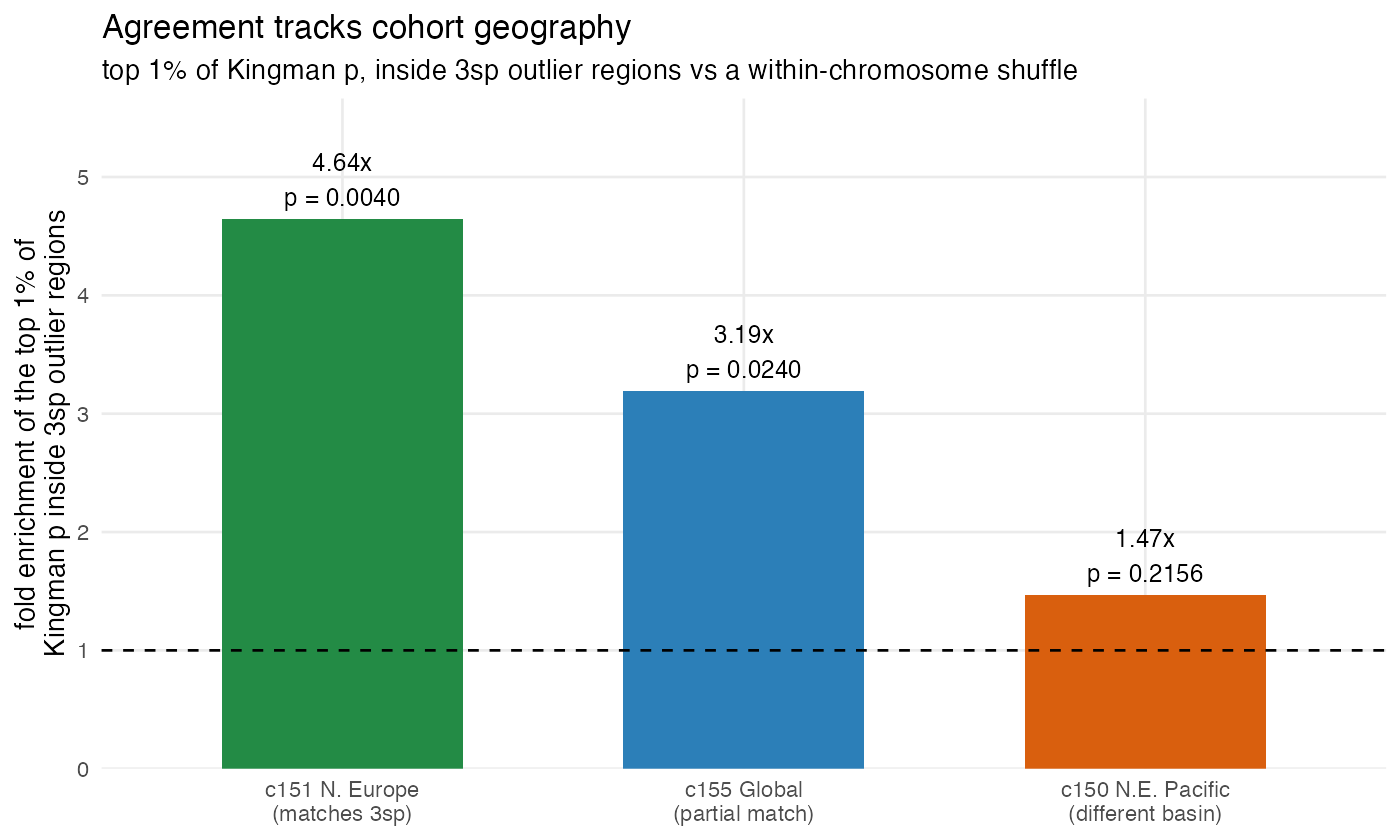
\includegraphics[width=0.62\textwidth]{../figures/fig3_geographic_gradient.png}
\caption{Agreement with the 3sp outlier regions tracks the geography of the Kingman cohort.}
\end{figure}

One honest qualification: the top-0.1\% column disagrees with the top-1\% column. c151's
1.70\,M $p$-values take only 19{,}035 distinct values, so its extreme tail is shaped by
which genotype configurations \emph{can} attain a low $p$ rather than by signal. The
top-1\% comparison is the trustworthy one.

\section{Which regions actually overlap}

\begin{table}[h]\centering\small
\begin{tabular}{llrl}\toprule
Region (gasAcu1) & Kingman peak & Overlap & Genes \\ \midrule
Chr1 21.499--21.929 & Global spec.\ ($p{=}4.5\mathrm{e}{-}15$) & 429\,kb & \gene{tns1, igfbp5, igfbp2a, stk11ip,} \\
                    & \emph{and} Pacific spec.\ ($8.8\mathrm{e}{-}12$) & & \gene{cx44.2, inha, spega, ctdsp1} \\
Chr16 16.479--16.829 & Pacific specific & 350\,kb & \gene{fer1l6, prkag3b, ttll4, abcb6b, kalrna, ahr1b} \\
Chr4 22.732--23.052 & Pacific specific & 320\,kb & \gene{large1, mkrn1, caprin2, ipo8} \\
Chr4 20.985--21.278 & Pacific specific & 293\,kb & \gene{slc2a13, iapp, pyroxd1, etnk1} \\
Chr4 21.542--21.746 & Pacific specific & 203\,kb & \gene{mapk11, mapk12b, lrig3, slc16a7} \\
Chr4 11.368--11.535 & Pacific specific & 167\,kb & \gene{rack1, ctbp1, spon2a} \\
Chr4 14.428--14.563 & Pacific specific & 134\,kb & \gene{gria1a, med7, itk, cyfip2} \\
Chr11 6.247--6.370  & Pacific specific & 123\,kb & \gene{mrc2, rnd2, vat1, phb} \\
Chr12 11.874--11.986 & Pacific specific & 112\,kb & \gene{rhocb, wnt2b} \\
Chr4 14.313--14.373 & Pacific specific & 61\,kb & \gene{foxi3a, wnt8a} \\
Chr14 11.353--11.362 & Global \emph{and} Pacific spec. & 9\,kb & \gene{cel} \\ \bottomrule
\end{tabular}
\end{table}

\subsection{The one locus everything agrees on}

\textbf{Chr1 21.499--21.929\,Mb} (gasAcu1) $=$ chrI 26.1--26.5\,Mb (gasAcu1-4) is recovered
by four independent routes: the 3sp LFMM regions, the 3sp EMMAX regions (where it is the
top region, 245 SNPs), the published Global-specific EcoPeak, and the c151
northern-European signal (its strongest suggestive peak). It is the Chr1 inversion.

\begin{figure}[h]\centering
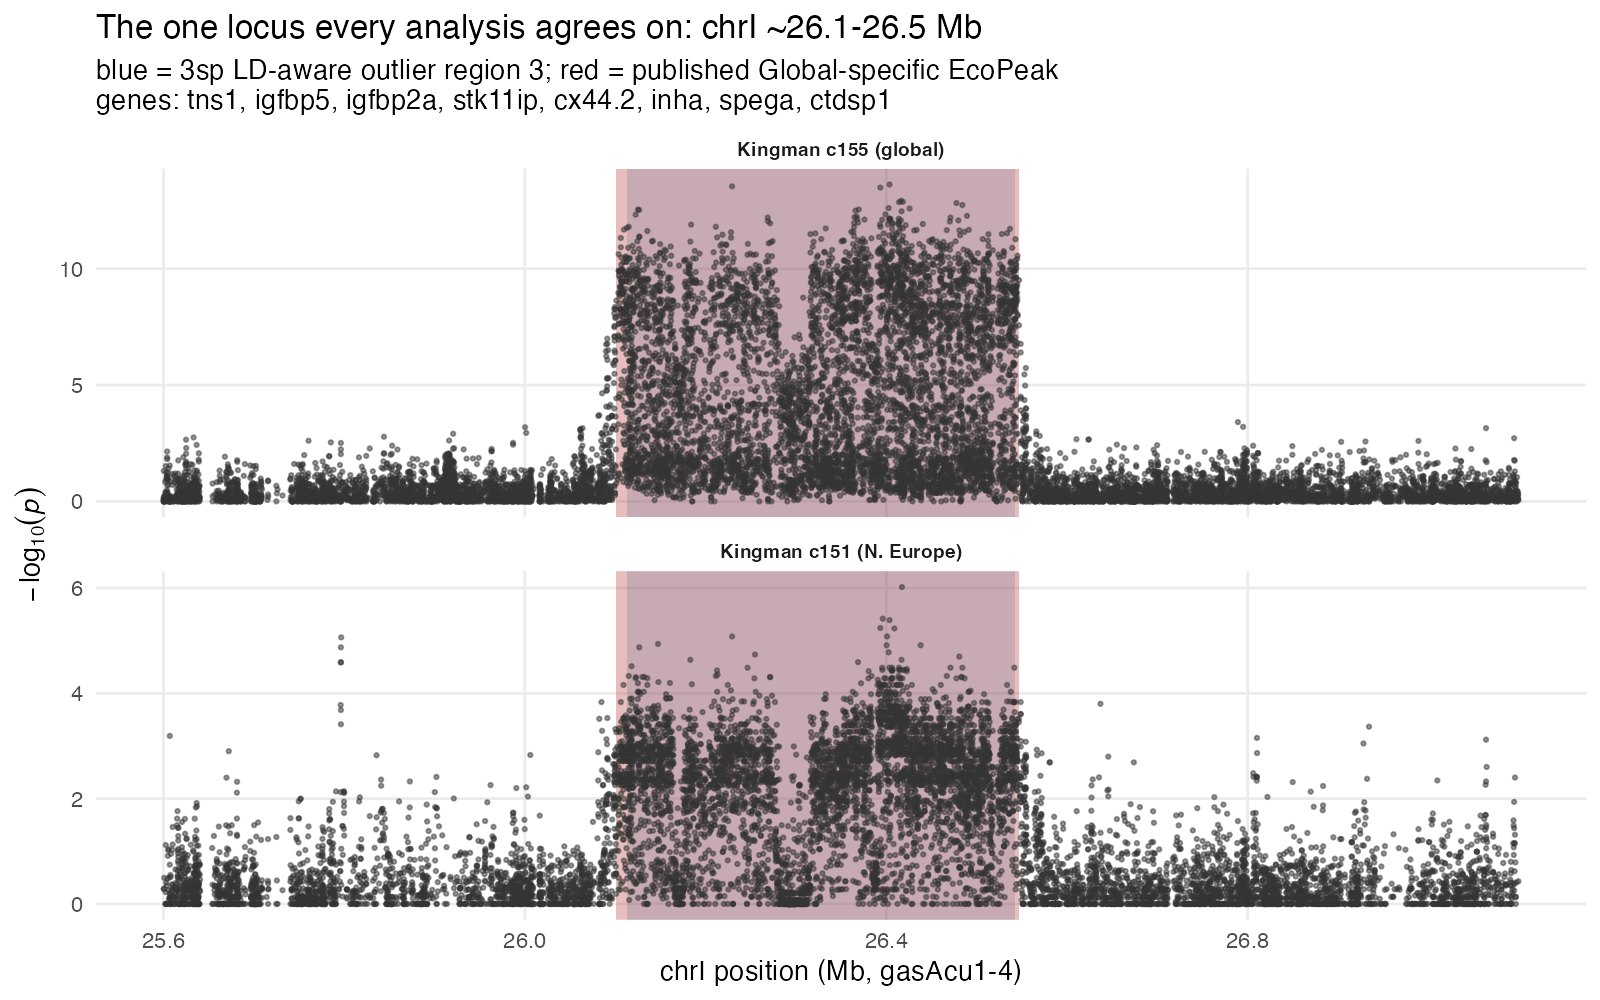
\includegraphics[width=0.8\textwidth]{../figures/fig4_chrI_locus.png}
\caption{The shared chrI locus in the two Kingman cohorts. The 3sp outlier region (blue)
and the published Global-specific EcoPeak (red) coincide so closely that the bands overlap.
The signal block is sharply bounded in both cohorts, and present in c151 despite that
cohort having no genome-wide-significant SNP anywhere.}
\end{figure}

\subsection{\gene{Eda}: recovered by EMMAX at $l_{\min}{=}3$, missed by LFMM entirely}
\label{sec:eda}

The \gene{Eda} gene sits at chrIV:12{,}812{,}613--12{,}822{,}840 (gasAcu1-4), i.e.\
12{,}800{,}219--12{,}810{,}446 in gasAcu1, squarely inside a published EcoPeak. In the
$l_{\min}{=}10$ LFMM set analysed above it falls in the \emph{gap} between region 9
(ending 12.284\,Mb) and region 10 (starting 14.034\,Mb), and the four $l_{\min}{=}10$
EMMAX regions contain no Chr4 entry at all --- which is what an earlier version of this
report recorded as a flat absence. That was too strong. Relaxing the cluster-size floor
resolves it, but only for one of the two methods:

\begin{table}[h]\centering\small
\begin{tabular}{llll}\toprule
Method & $l_{\min}$ & \gene{Eda} recovered? & Why \\ \midrule
EMMAX & 3  & \textbf{yes} & region 7 = Chr4:12{,}809{,}075--12{,}811{,}617, \textbf{4 SNPs} \\
EMMAX & 10 & no & the same region has only 4 SNPs, below the floor \\
LFMM  & 3  & no & Chr4 regions jump 12.284 $\rightarrow$ 14.034\,Mb \\
LFMM  & 10 & no & same gap \\ \bottomrule
\end{tabular}
\end{table}

The recovered EMMAX region overlaps the \gene{eda} gene body by \textbf{1{,}371\,bp}, and
sits inside the Global-specific EcoPeak carrying the \emph{most extreme SNP $p$-value in
that entire set} ($7.9\times10^{-15}$; the matching Pacific-specific peak is
$2.2\times10^{-12}$).

Two things follow. First, this is a \textbf{method difference, not merely a threshold
choice}: LFMM does not find \gene{Eda} at either cluster-size floor, so lowering
$l_{\min}$ alone does not rescue it. Second, it vindicates the claim in
\texttt{module\_sticklebacks\_LDscnR/README.md} that the C-score resolves Chr4/\gene{Eda}
--- the earlier report was simply reading it off the wrong region set. \gene{Eda} is a
4-SNP cluster, so any analysis that demands $\geq$10 linked SNPs will discard the textbook
marine--freshwater locus. That is a cautionary result about $l_{\min}$ in its own right.

\section{The $l_{\min}{=}3$ region sets}\label{sec:lmin3}

The analysis above uses the 40 LFMM $l_{\min}{=}10$ regions. The main manuscript's
structure-null analysis instead works from $l_{\min}{=}3$ sets, so the overlap was recomputed
on those (\texttt{R/12}, \texttt{R/13}, \texttt{R/15}). The three sets differ enormously in
how much genome they claim:

\begin{table}[h]\centering\small
\begin{tabular}{llrrrrr}\toprule
Set & $l_{\min}$ & Regions & Span & Global-spec.\ hit & Fold & $p$ \\ \midrule
\textbf{EMMAX} & 3  & 17  & \textbf{1.21\,Mb}  & \textbf{5/17}   & \textbf{19.5$\times$} & \textbf{0.0005} \\
LFMM           & 10 & 40  & 21.13\,Mb          & 4/40            & 1.38$\times$          & 0.33 \\
LFMM           & 3  & 136 & 37.27\,Mb          & 9/136           & 1.87$\times$          & 0.036 \\ \bottomrule
\end{tabular}
\end{table}

The EMMAX $l_{\min}{=}3$ set is the standout: 17 regions covering 1.21\,Mb --- 0.3\% of the
genome --- of which 5 land on the 39 Global-specific EcoPeaks, \textbf{19.5$\times$ over a
within-chromosome rotation null}. Against the Pacific-specific set it is 5/17,
2.36$\times$, $p = 0.039$; against the sensitive sets 7/17 (4.61$\times$) and 8/17
(1.48$\times$, n.s.). The LFMM $l_{\min}{=}3$ set covers 30$\times$ more genome for a
1.87$\times$ enrichment, so the difference is precision, not coverage.

\begin{figure}[h]\centering
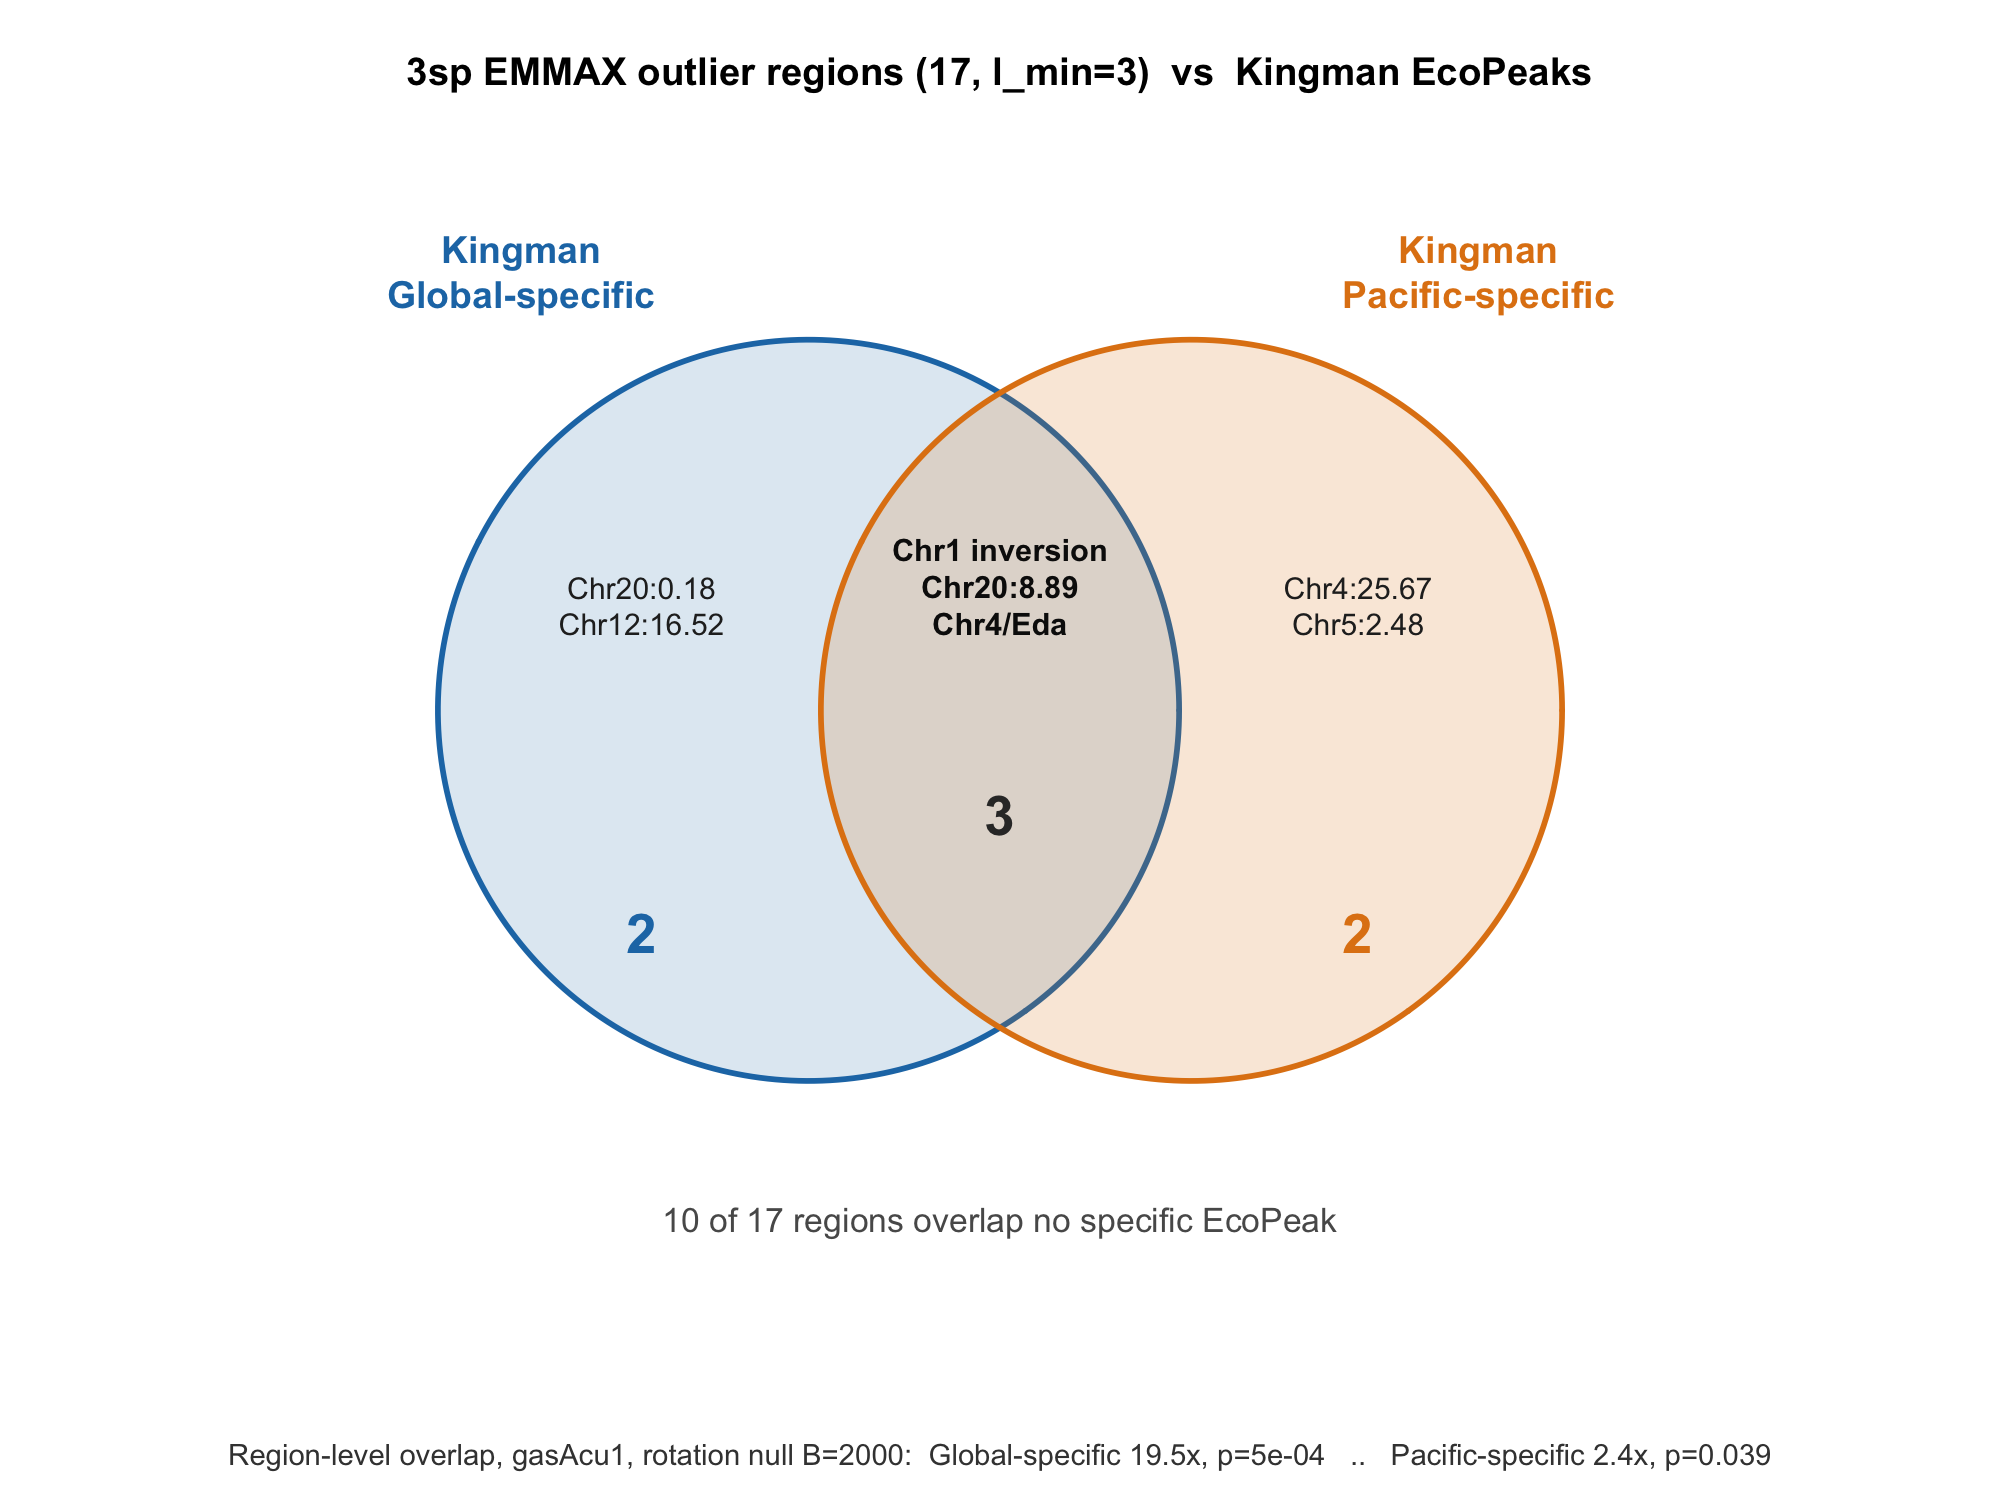
\includegraphics[width=0.72\textwidth]{../figures/fig5_venn_emmax17.png}
\caption{Which of the 17 EMMAX $l_{\min}{=}3$ regions hit which specific EcoPeak set.
Three regions hit both --- the Chr1 inversion, Chr20:8.89\,Mb, and Chr4/\gene{Eda}
(\S\ref{sec:eda}). Ten of 17 hit no specific EcoPeak.}
\end{figure}

\begin{figure}[h]\centering
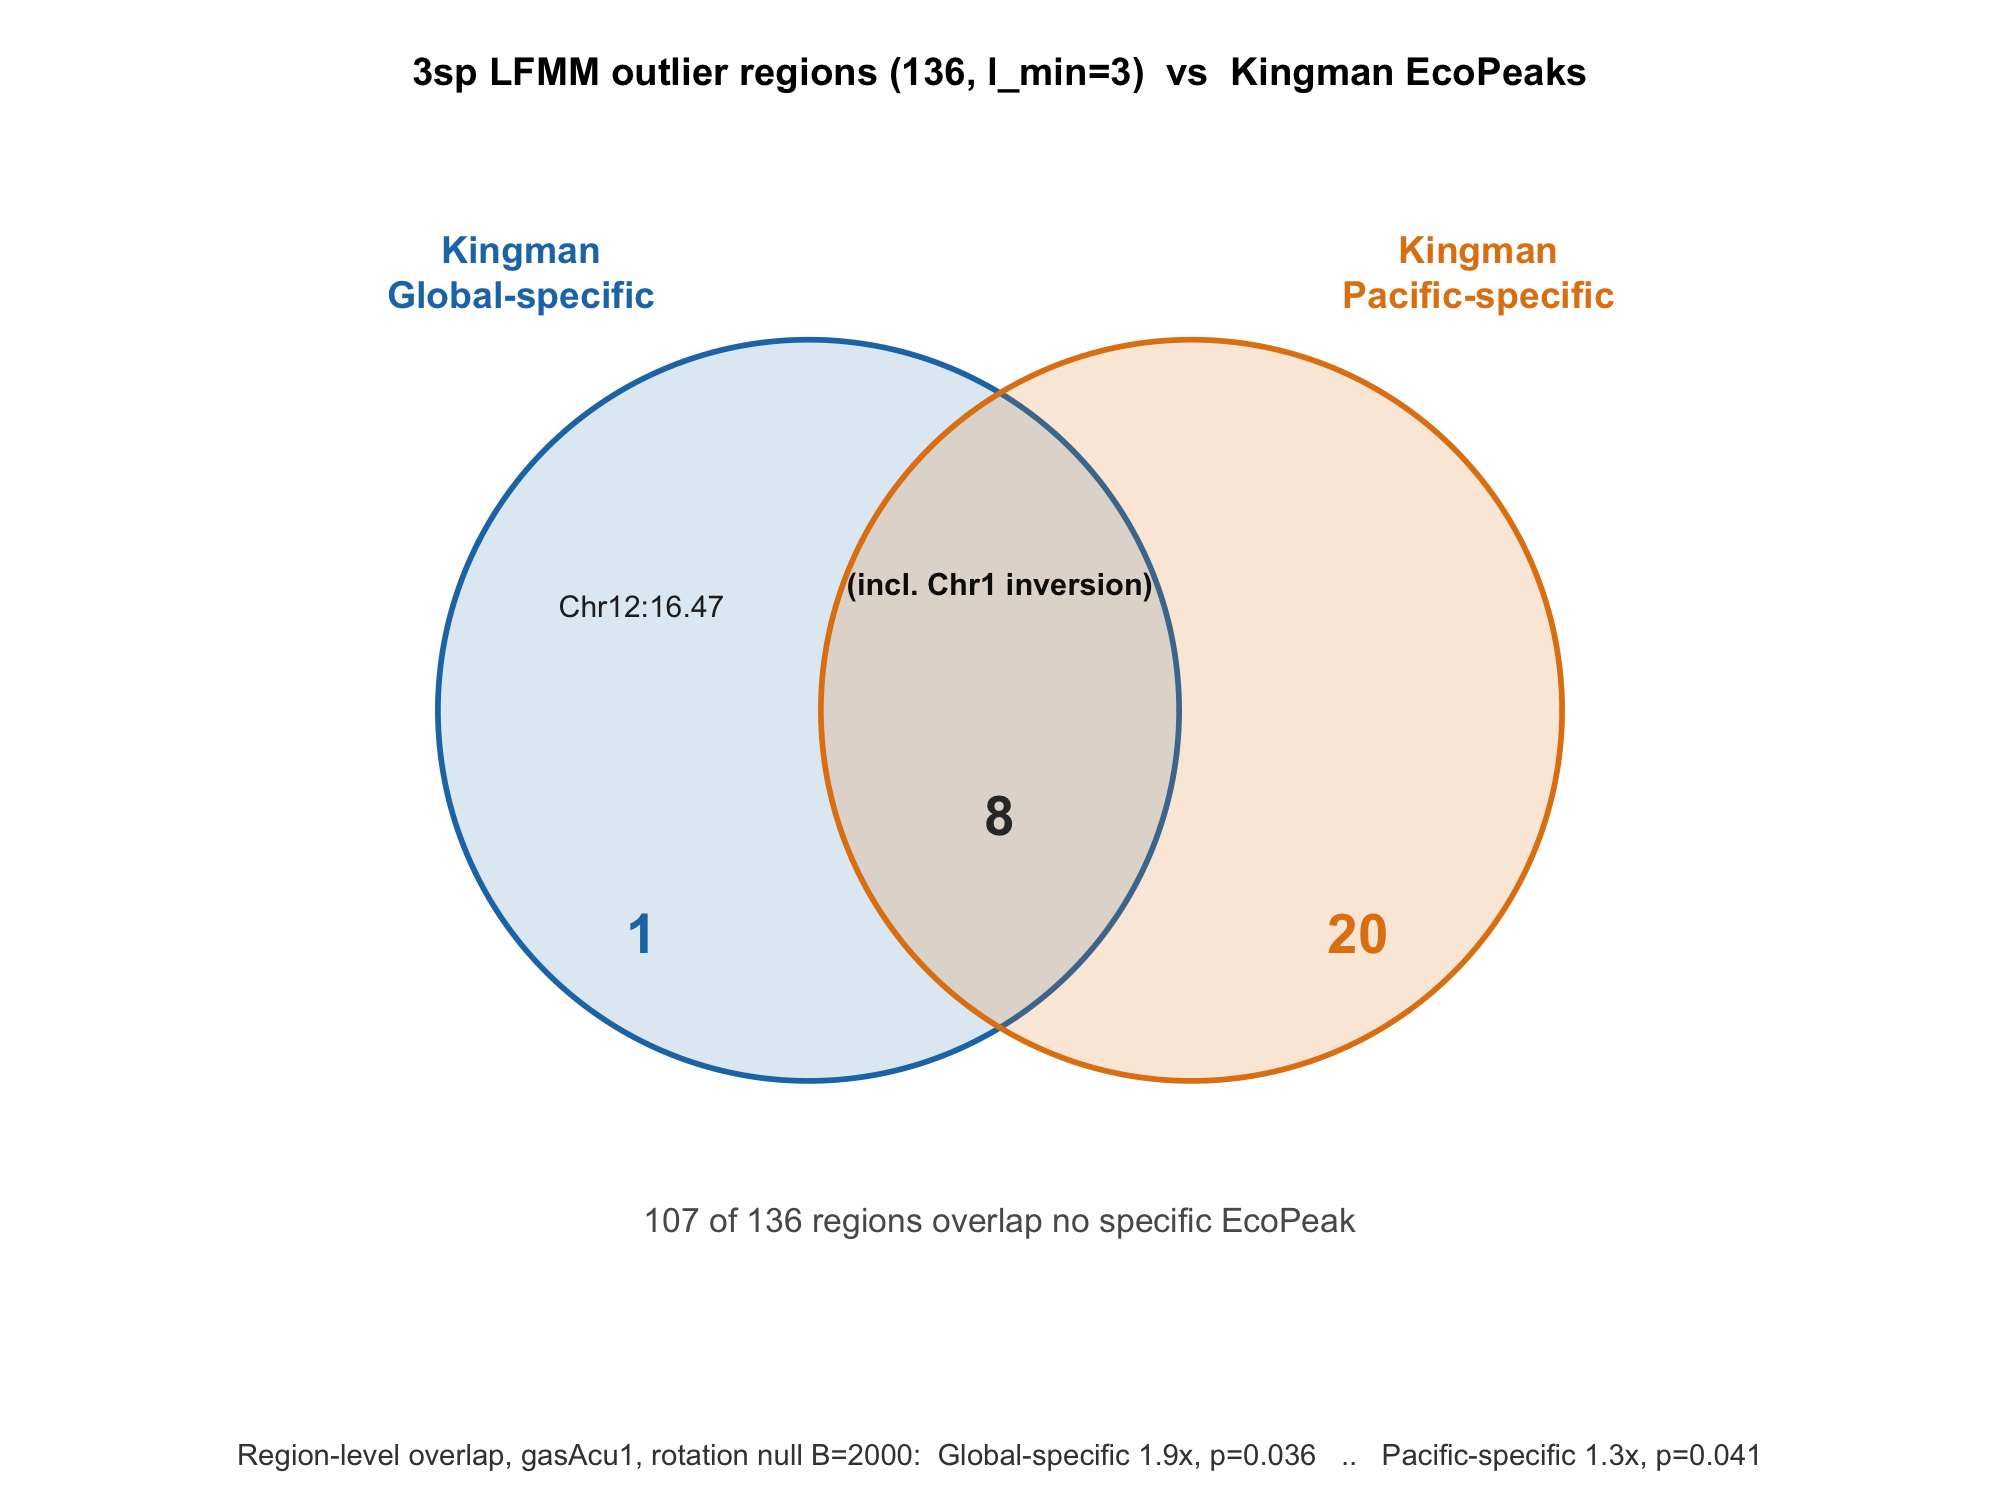
\includegraphics[width=0.72\textwidth]{../figures/fig5_venn_lfmm.png}
\caption{The same view for the 136 LFMM $l_{\min}{=}3$ regions, for contrast. Only 29 of
136 hit any specific EcoPeak and 107 hit none; of the nine touching the Global-specific
set, eight also touch the Pacific-specific set. Note the asymmetry against
Fig.~5: the LFMM set finds \emph{more} Pacific-only regions (20 vs 2) but adds almost
nothing Global-only (1 vs 2), while spending 37.27\,Mb to do it against the EMMAX set's
1.21\,Mb.}
\end{figure}

Rank-based enrichment of low Kingman $p$ inside the 17 regions, and the c151 suggestive-peak
overlap, both strengthen accordingly:

\begin{table}[h]\centering\small
\begin{tabular}{lrrrr}\toprule
Kingman cohort & top 1\% & $p$ & top 0.1\% & $p$ \\ \midrule
\texttt{c151} N. Europe    & \textbf{34.1$\times$} & 0.0020 & 11.3$\times$ & 0.026 \\
\texttt{c155} Global       & 25.9$\times$ & 0.0040 & \textbf{33.5$\times$} & 0.0060 \\
\texttt{c150} N.E. Pacific & 17.6$\times$ & 0.0020 & 11.1$\times$ & 0.016 \\ \bottomrule
\end{tabular}
\end{table}

c151 suggestive peaks inside the 17 regions: 5 of 41 against 0.33 expected,
\textbf{15.1$\times$, $p = 0.0002$}.

\textbf{Two cautions on reading these numbers.} They are \emph{not} comparable to the
$l_{\min}{=}10$ folds in \S\ref{sec:geo}: fold enrichment scales inversely with how much
genome a region set claims, and 1.21\,Mb of tightly targeted regions will always out-fold
19.92\,Mb of broad ones. 34$\times$ here versus 4.64$\times$ there does not mean the EMMAX
set agrees seven times better. And the \textbf{geographic gradient reproduces only in the
top-1\% column} (c151 $>$ c155 $>$ c150); in the top-0.1\% column c155 is highest, exactly
as it was for the $l_{\min}{=}10$ set. That is consistent across both region sets and has a
straightforward reading: c155 is much the best-powered cohort (84 samples, 28 marine) and so
produces the most extreme $p$-values, meaning the extreme tail ranks statistical power
rather than geography. The top-1\% comparison is where geography shows.

\section{How much agreement is even achievable?}\label{sec:ceiling}

A partial overlap only means something against a ceiling. The natural ceiling is Kingman's
own two published peak sets: if Global-specific and Pacific-specific --- same laboratory,
same VCF, same caller, differing only in which populations enter the cohort --- agree only
loosely with each other, then loose agreement with a 3sp region set is the expected result
rather than a shortfall.

The comparison must not be made with fold enrichment, whose ceiling differs for every pair
(a set covering 0.3\% of the genome can reach 64$\times$; one covering 5.6\% saturates near
4$\times$). Nor with the Jaccard index, which is capped by the span ratio of the two sets.
The fair measure is the \textbf{overlap coefficient}, bp intersection over the bp of the
\emph{smaller} set: 1.0 means the smaller claim is entirely corroborated by the larger.

\begin{table}[h]\centering\small
\begin{tabular}{llrrrrr}\toprule
Set A & Set B & Span A & Span B & $\cap$ & \textbf{Overlap coef.} & $p$ \\ \midrule
\multicolumn{7}{l}{\emph{within a dataset}}\\
3sp EMMAX $l_{\min}{=}3$ & 3sp LFMM $l_{\min}{=}3$ & 1.21 & 37.27 & 1.158 & \textbf{0.959} & 0.0005 \\
Kingman Global-spec & Kingman Pacific-spec & 3.52 & 24.96 & 3.340 & \textbf{0.950} & 0.0005 \\
Kingman Global-sens & Kingman Pacific-sens & 22.09 & 82.68 & 20.972 & 0.949 & 0.0005 \\
3sp EMMAX $l_{\min}{=}3$ & 3sp LFMM $l_{\min}{=}10$ & 1.21 & 21.13 & 1.046 & 0.865 & 0.0005 \\ \midrule
\multicolumn{7}{l}{\emph{across datasets}}\\
3sp EMMAX $l_{\min}{=}3$ & Kingman Pacific-spec & 1.21 & 24.96 & 0.536 & 0.444 & 0.037 \\
3sp EMMAX $l_{\min}{=}3$ & Kingman Global-spec & 1.21 & 3.52 & 0.497 & 0.411 & 0.0005 \\
3sp LFMM $l_{\min}{=}3$ & Kingman Global-spec & 37.27 & 3.52 & 0.972 & 0.277 & 0.049 \\
3sp LFMM $l_{\min}{=}3$ & Kingman Pacific-spec & 37.27 & 24.96 & 4.792 & 0.192 & 0.046 \\
3sp LFMM $l_{\min}{=}10$ & Kingman Pacific-spec & 21.13 & 24.96 & 3.173 & 0.150 & 0.028 \\
3sp LFMM $l_{\min}{=}10$ & Kingman Global-spec & 21.13 & 3.52 & 0.476 & 0.135 & 0.32 \\ \bottomrule
\end{tabular}
\end{table}

\textbf{Kingman's two datasets are essentially nested: 95\% of the Global-specific sequence
lies inside the Pacific-specific set}, and the same for the sensitive pair. Their internal
consistency is near-total --- the Global peaks are, to a very good approximation, the
stringent subset of the Pacific peaks. That is a high ceiling.

Our best cross-dataset figure is \textbf{0.444}, less than half of it. So the honest reading
is that the 3sp region sets are \emph{not} reproducing Kingman at the limit of what is
achievable; there is a real gap, and \S\ref{sec:geo} argues it is largely geographic.

One number does match the ceiling, but it is not the one that would flatter us. Our two
methods agree with \emph{each other} at 0.959 --- the EMMAX $l_{\min}{=}3$ regions are
almost entirely nested inside the LFMM $l_{\min}{=}3$ regions --- marginally above Kingman's
own 0.950. That is a within-dataset comparison, so it is not the same kind of quantity: it
says the two 3sp scans are internally consistent, not that they agree with Kingman. And the
containment is over a wider span ratio (1.21\,Mb inside 37.27\,Mb, versus 3.52 inside
24.96), which makes nesting easier. The honest summary is that \textbf{no analysis of ours
agrees with Kingman as well as Kingman's two datasets agree with each other.}

All figures come from \texttt{R/10\_figures.R} and every number in this report is read from \texttt{data/overlap\_summary.csv}, \texttt{data/enrichment\_summary.csv}, \texttt{data/c151\_peak\_overlap.csv} and \texttt{data/overlap\_detail.csv}, all regenerated by \texttt{R/09\_overlap.R} and \texttt{R/11\_c151\_peak\_overlap.R}. The
$l_{\min}{=}3$ results of \S\ref{sec:lmin3} come from \texttt{data/overlap\_summary\_emmax17.csv},
\texttt{data/overlap\_summary\_lfmm.csv}, \texttt{data/enrichment\_emmax17.csv} and
\texttt{data/c151\_peak\_overlap\_emmax17.csv} (\texttt{R/12}, \texttt{R/13}, \texttt{R/15}),
with Figs.~5--6 from \texttt{R/14\_venn\_emmax17.R} (run as \texttt{emmax17} and \texttt{lfmm}).
\S\ref{sec:ceiling} is \texttt{data/peakset\_concordance.csv} from \texttt{R/16\_peakset\_concordance.R}.

\section{Using the EcoPeaks to calibrate, not just to score}\label{sec:calib}

Everything above uses the EcoPeaks to \emph{score} a fixed region set. They can also be
used to \emph{calibrate}: sweep the $\tau_C \times \ell_{\min}$ grid that produces the
3sp regions, and ask which cell best recovers an external truth. Two findings came out of
doing that, one methodological and one about the two scan engines.

\subsection{Most of the grid cannot support the statistic}

Two of the four natural scores --- precision (fraction of a cell's regions that hit an
EcoPeak) and fold over a rotation null --- divide by the number of regions in the cell.
When a cell holds one region that happens to hit, precision is $1.0$ and the fold is
whatever the near-empty null allows, which on this grid reached $200\times$. Left
unmasked these degenerate cells form a bright band across the high-$\tau_C$,
high-$\ell_{\min}$ corner and invert the apparent optimum.

Masking cells with fewer than five regions is therefore not cosmetic. It is severe for
EMMAX --- \textbf{only $33$ of $270$ cells survive} --- and mild for LFMM, where $247$ survive.
That contrast is itself the most informative number in the sweep, and \S\ref{sec:engines}
returns to it.

\begin{table}[h]\centering\small
\begin{tabular}{lrllr}\toprule
Sweep & Estimable & F1-optimal cell & $F_1$ (max / at $\tau_C{=}0.05,\ell_{\min}{=}3$) & Rank \\ \midrule
EMMAX / global-spec  & 33/270  & $\tau_C{=}0.10$, $\ell_{\min}{=}1$ & 0.197 / 0.189 & 3 \\
EMMAX / Pacific-spec & 33/270  & $\tau_C{=}0.05$, $\ell_{\min}{=}1$ & 0.092 / 0.048 & 2 \\
LFMM / global-spec   & 247/270 & $\tau_C{=}0.10$, $\ell_{\min}{=}6$ & 0.135 / 0.102 & 15 \\
LFMM / Pacific-spec  & 247/270 & $\tau_C{=}0.05$, $\ell_{\min}{=}5$ & 0.217 / 0.212 & 4 \\ \bottomrule
\end{tabular}
\end{table}

The operating point $\tau_C = 0.05$, $\ell_{\min} = 3$ is \emph{not} the F1 maximum in any
of the four, though it is close in three. On the masked grid precision does peak in the
low-$\tau_C$ corner ($0.40$ at $\tau_C = 0.05$, $\ell_{\min} = 6$--$9$), but fold does not
--- it favours the $\ell_{\min} = 1$ edge at high $\tau_C$ ($46\times$ at $\tau_C = 0.70$),
in cells sitting at the masking floor. Recall is capped near $0.28$ by biology rather than
by the threshold, since most global EcoPeaks are Pacific-derived and absent from an
Atlantic panel, so F1 --- half of which is recall --- should not be treated as the
objective. Precision is the axis on which the chosen point is close to the best available.

\begin{figure}[h]\centering
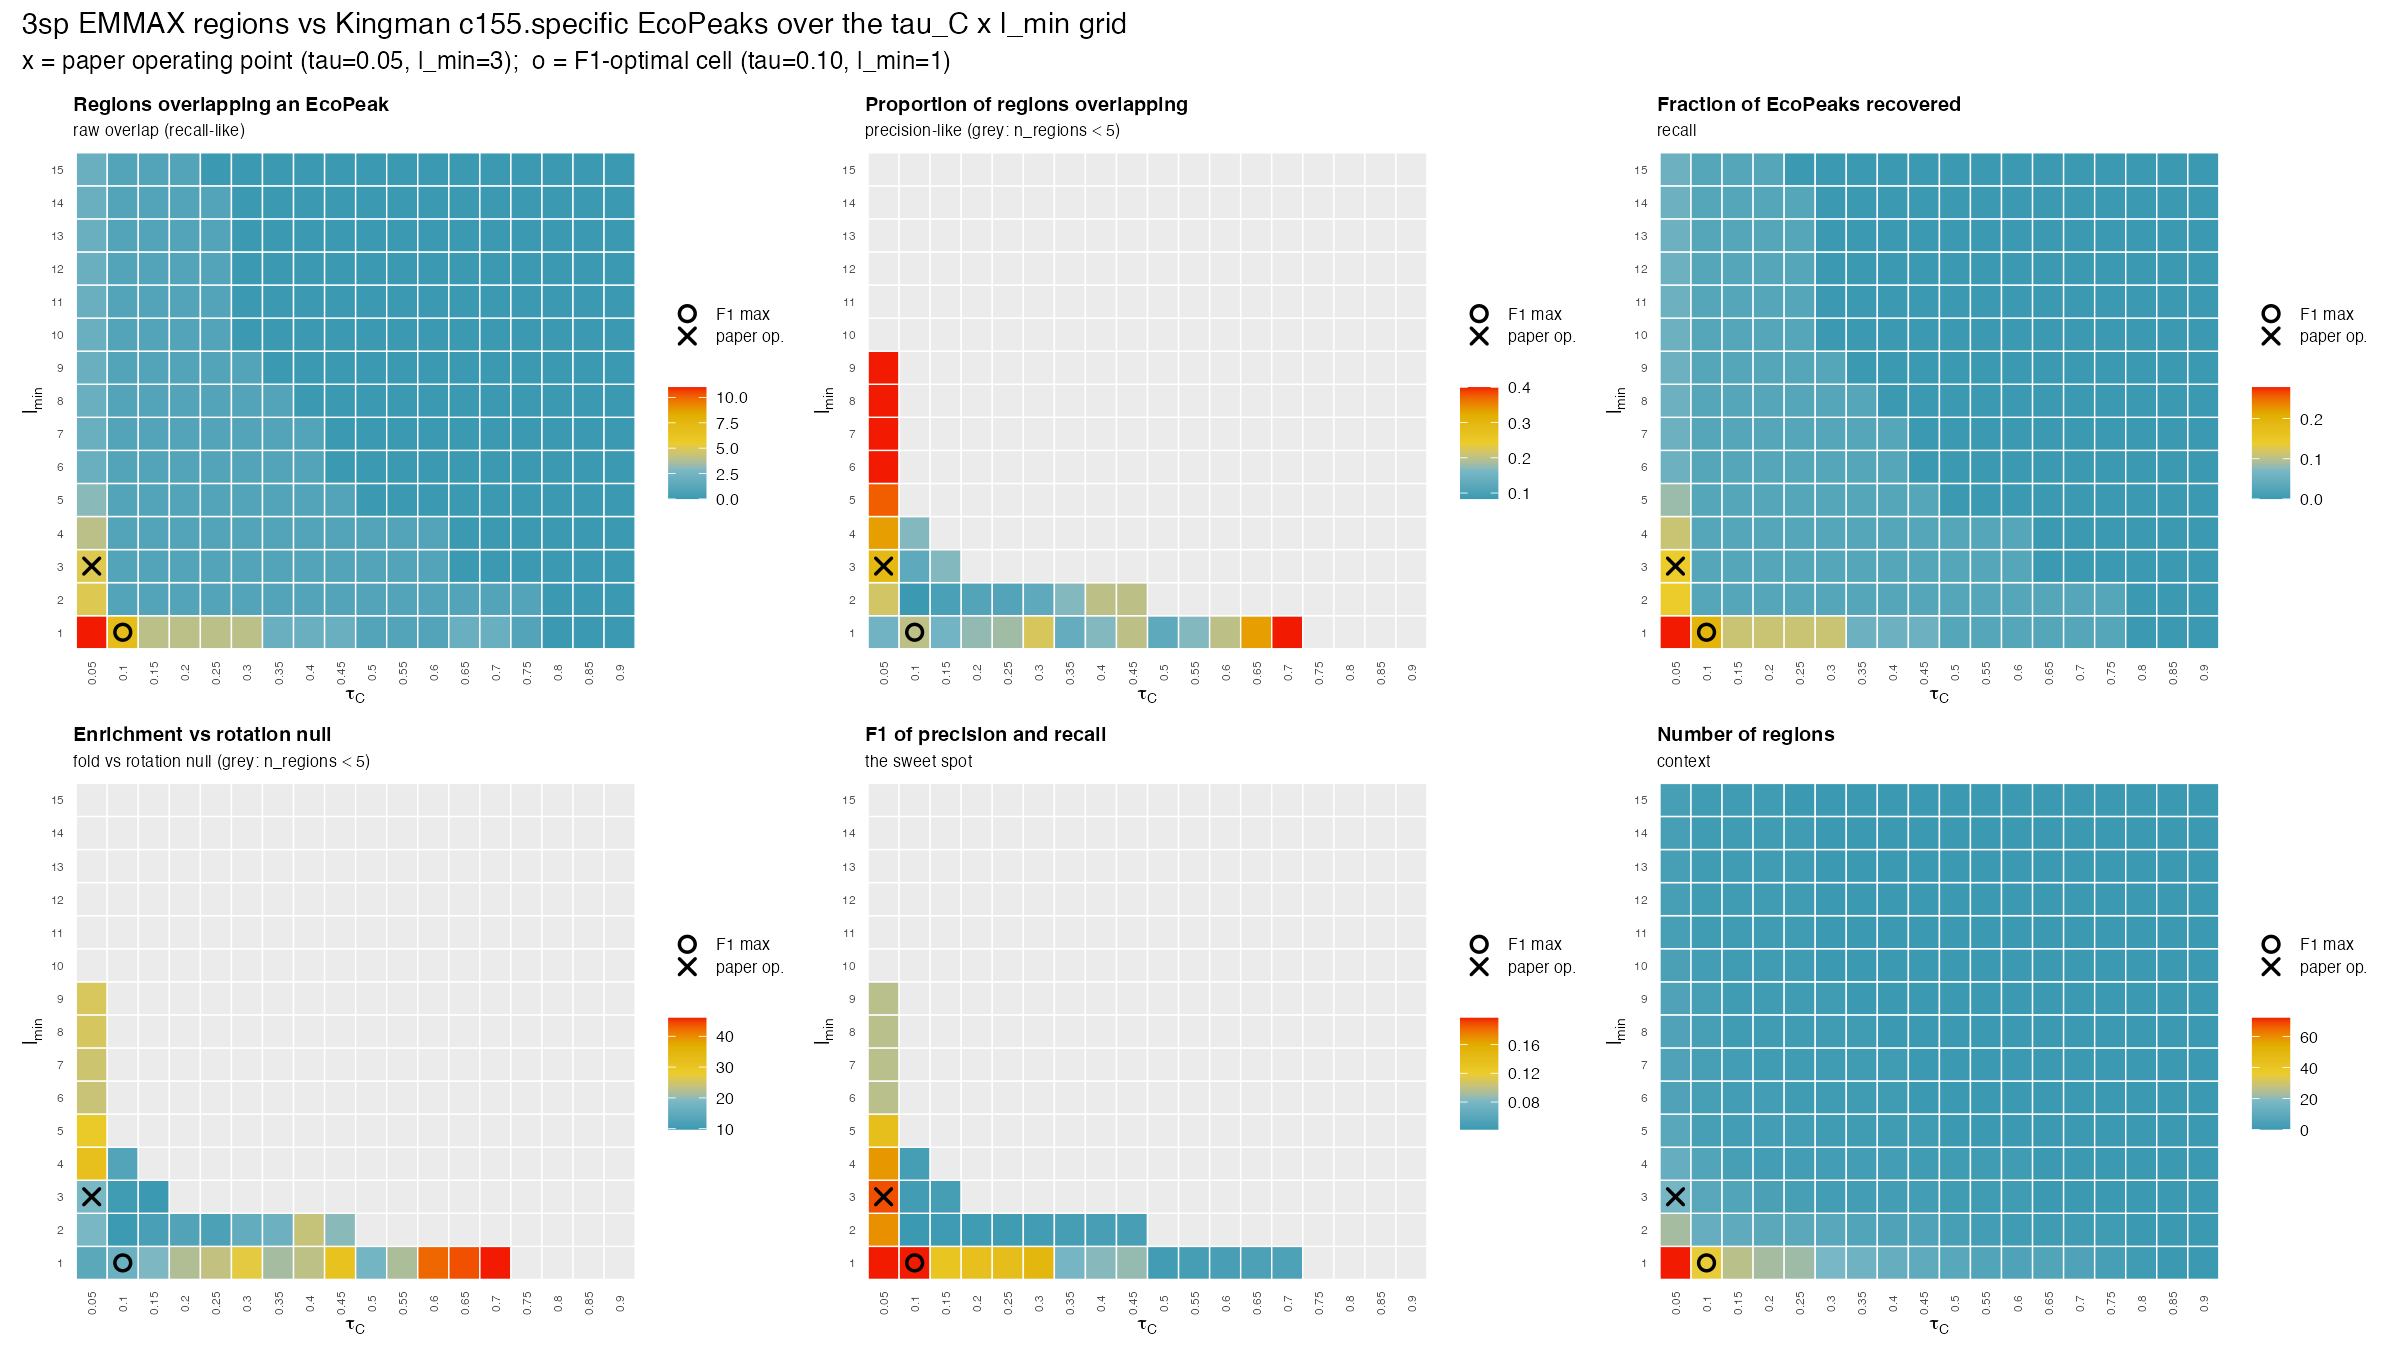
\includegraphics[width=\textwidth]{../figures/fig7_sweep_emmax.png}
\caption{The $\tau_C \times \ell_{\min}$ sweep scored against the Global-specific
EcoPeaks. Grey cells hold fewer than five regions, where precision, fold and F1 are not
estimable. The cross is the operating point, the circle the F1 maximum.}
\end{figure}

\subsection{What the sweep says about the two engines}\label{sec:engines}

The estimable-cell counts ($33$ for EMMAX, $247$ for LFMM) say that $C$ discriminates very
differently in the two scans. Following $\ell_{\min} = 3$ across the grid:

\begin{center}\small
\begin{tabular}{lrrrrr}\toprule
Regions at $\tau_C =$ & 0.05 & 0.10 & 0.30 & 0.60 & 0.90 \\ \midrule
EMMAX & 17 & 8 & 2 & 1 & 0 \\
LFMM & 136 & 133 & 107 & 84 & 29 \\ \bottomrule
\end{tabular}
\end{center}

EMMAX falls out of the estimable range almost immediately; LFMM still holds $84$ regions at
$\tau_C = 0.60$. This matches the per-SNP picture: \textbf{$782$ LFMM SNPs carry
$C > 0.5$ against EMMAX's $13$}. A large block of LFMM SNPs passes in nearly every
$(\rho, q^*)$ cell, so almost any threshold retains them.

Crucially, no threshold rescues them. Across every estimable $\tau_C$ at $\ell_{\min} = 3$,
LFMM's precision stays in $0.029$--$0.068$ and its fold in $1.8$--$6.4$, against EMMAX's
$0.125$--$0.294$ and $9.7$--$18.8$ over its three estimable cells. The LFMM regions are not
the right regions at the wrong threshold; the ranking does not track the external truth
anywhere on the grid.

\subsection{The per-SNP C-score, and what it is not}

Binning every SNP by $C$ and measuring Global-specific EcoPeak membership
(Fig.~\ref{fig:cscore}), the informative signal is the \emph{step} from $C = 0$ to
$C > 0$. EMMAX SNPs with any $C > 0$ are enriched $24$--$53$-fold over the $1.31\%$
genome-wide rate, while the ${\sim}789{,}000$ SNPs at $C = 0$ sit at background
($0.91\times$). Within $C > 0$, however, \emph{neither} method rises: EMMAX peaks in the
$(0.05, 0.1]$ bin and falls to $23.5\times$ at the top, LFMM falls monotonically from
$21.7\times$ to $3.8\times$. The positive rank correlations (Spearman $\rho = 0.21$ EMMAX,
$0.06$ LFMM) restate the step and are not evidence of a graded trend, since the $C = 0$
class dominates both. $C$ should be read as a candidate flag, not as a finely graded
strength of evidence.

What separates the engines is the top of the scale: at $C > 0.5$ EMMAX places $13$ SNPs
still enriched $23.5\times$, LFMM places $782$ enriched $3.8\times$.

\begin{figure}[h]\centering
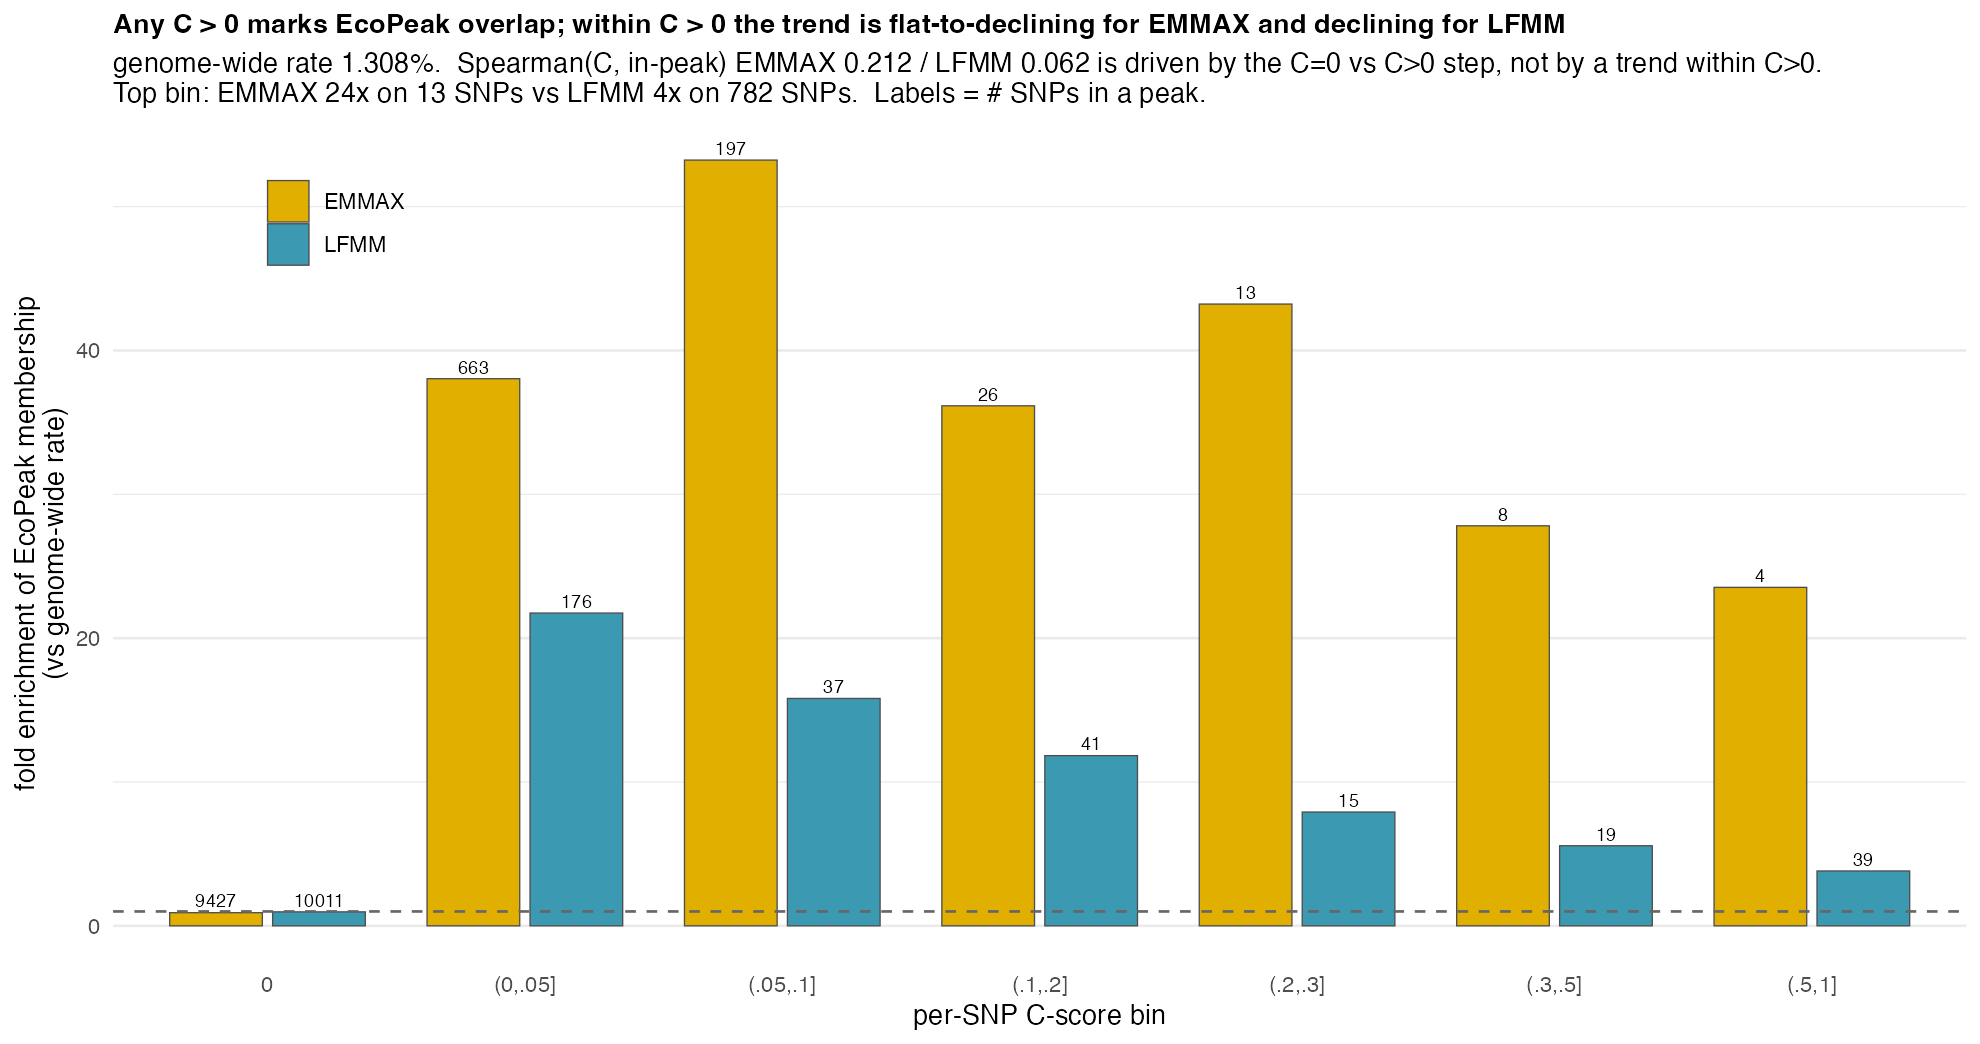
\includegraphics[width=\textwidth]{../figures/fig8_cscore.png}
\caption{Per-SNP C-score versus Global-specific EcoPeak membership.}
\label{fig:cscore}
\end{figure}

\subsection{A caution: LFMM has no structure-aware null}\label{sec:lfmmnull}

The asymmetry above should be read with one confound in view. The EMMAX arm is calibrated
by a structure-aware null; the LFMM arm has none, and its $\tau_C$ is transferred from
EMMAX. Attributing the whole difference to the engines is therefore not clean.

Two observations bear on it. First, LFMM is \emph{not} inflated in the usual sense:
$\lambda_{GC} = 1.008$ against EMMAX's $1.093$, because the LFMM test applies genomic
control and forces the median to calibration. What it has is a heavy \emph{tail} --- $207$
SNPs at $p < 10^{-6}$ against EMMAX's $13$, and $952$ at BH $q < 0.05$ against $3$.
Describing this as an inflated baseline would be wrong; the baseline is calibrated and the
tail is not.

Second, the sweep and a null answer different questions. The sweep shows LFMM's $C$ does
not \emph{rank} SNPs in a way that tracks the EcoPeaks. A null would show whether LFMM's
$C$ values are unusual \emph{at all} against permuted ecotype. These can dissociate, and
the interesting outcome is that they do: LFMM could pass its negative control --- every
region far above null --- while failing the positive control. That would mean LFMM detects
something real and structured that is not recurrent marine--freshwater adaptation.

The direction is not predictable from what is in hand, because an among-population ecotype
permutation breaks the ecotype--population correlation, and if LFMM's heavy tail derives
from that correlation the null will be low and its regions will clear it comfortably. This
is the main open item left by this module. A small run ($B \approx 5$--$10$ surrogates)
would settle the direction, since what matters first is whether the null $C$ distribution
piles up near $1$ or collapses toward $0$; a full $B$ is only needed for per-region
$p$-values.

\section{Caveats}

\begin{itemize}\itemsep2pt
\item Only the SNP-based half of Kingman's two-method peak caller is implemented; the
      derived sets are sensitive supersets of "specific".
\item \texttt{GTs} is mean-imputed at 5.5$\times$ coverage; expect $r^2$/\texttt{ld\_w}
      attenuation.
\item 3sp region boundaries are the min/max SNP position of an LD cluster, hence coarse.
\item 3 of 39 global-specific peaks lift to \texttt{chrUn} and 1 sits on \texttt{chrXIX},
      which 3sp drops, leaving 36 comparable.
\item c151 results are rank-based and carry no FDR guarantee.
\item The sweep of \S\ref{sec:calib} masks cells below five regions; the floor is a
      pragmatic choice, not a derived threshold.
\item LFMM has no structure-aware null here, so the engine comparison is confounded
      (\S\ref{sec:lfmmnull}).
\item Fold enrichments are not comparable between region sets of different total span
      (1.21\,Mb for EMMAX $l_{\min}{=}3$ vs 21.13\,Mb for LFMM $l_{\min}{=}10$); compare
      $p$-values and hit counts, not folds.
\item $l_{\min}$ is consequential, not cosmetic: \gene{Eda} is a 4-SNP cluster and is
      discarded by any $l_{\min}{\geq}10$ analysis (\S\ref{sec:eda}).
\item The recombination map leaves 3.6\% of SNPs without a \texttt{rec\_rate}.
\end{itemize}

\end{document}
